\documentclass[../main.tex]{subfiles}

\begin{document}

\section{Combinación de cargas}

Para la combinación de cargas, lo primero que se recomienda es la trasmisión
de \textbf{estados base}, y a partir de los mismos, calcular los esfuerzos 
últimos. Las combinaciones utilizadas son las dadas en CIRSOC 301 \textbf{Art. A.4.2}
como se muestra a continuación:

\begin{align*}
  &1.4 * (D) \\[5pt]
  &1.2 D + 1.6 L\\[5pt]
  &0.9 D +  1.6 W 
.\end{align*}

Por otro lado, para las cargas de servicio, utilizamos:

\begin{align*}
  &1*D + 1*W \\[5pt]
  &1*D + 1*L \\[5pt]
  &1*D + 0.7*(W+L) 
.\end{align*}

\section{Elementos de unión}

Podemos estudiar dos tipos de uniones: \textbf{abulonadas} y \textbf{soldadas}.
En nuestro caso, resolvimos principalmente ejercicios de uniones abulonadas.
Vamos a considerar las uniones abulonadas.

\subsection{Uniones abulonadas}

Lo primero es distinguir los dos tipos de bulones:

\begin{itemize}
  \item Bulones comunes calibrados. ($F_u=\SI{370}{MPA}$,$F_y\SI{235}{MPa}$)
  \item Bulones de alta resistencia. (\textit{varia})
\end{itemize}

\begin{figure}[htpb]
  \centering
  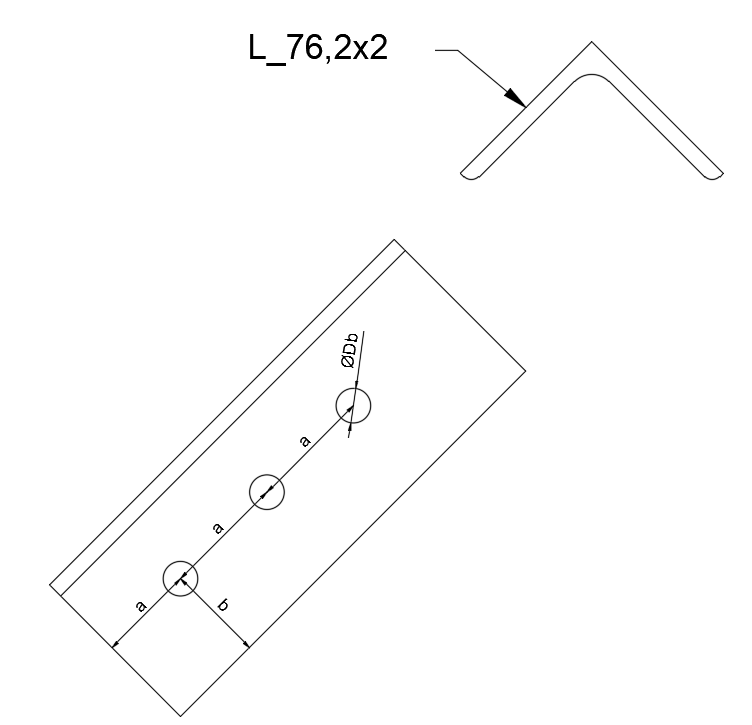
\includegraphics[width=0.6\textwidth]{../images/resumen/perfil}
  \caption{Perfil L}
  \label{fig:perfil}
\end{figure}

Lo primero que debemos hacer es encontrar los datos geométricos para resolver
el problema. Tomando, por ejemplo, un perfil L76.2x2 como se ve en \Cref{fig:perfil}
de tablas como la PentaKa, podemos obtener:

\begin{align*}
  B &= \SI{76.2}{mm} \tag{Ancho} \\[5pt]
  A_b &= \SI{2.98}{cm^2} \tag{Área bruta} \\[5pt]
  x_g &= \SI{2}{mm} \tag{Centro de gravedad}
.\end{align*}

Lo primero que debemos es encontrar el área a utilizar. Distinguimos tres tipos
de área: área bruta, área neta y área efectiva. El área neta $A_n$ es el área
bruta descontando los bulones, y el área efectiva  $A_e$ es el área teniendo en
cuenta el efecto llamado  \textit{retraso de cortante}, debido a que no todos 
los elementos están directamente conectados.

\subsubsection{Área efectiva}

En nuestro caso tenemos elementos no directamente conectados, por lo tanto
debemos encontrar el área efectiva. Esto se puede encontrar mediante la fórmula
\textbf{B.3.1.} del CIRSOC 301. Esta es:
\begin{align*}
  A_e = A_n * U
.\end{align*}

Donde U es un factor que debe ser obtenido, y que depende de la distancia 
$\overline{x}$, que es la distancia entre el plano de la unión y el centro de 
la unión. Esto se puede ver en la \textbf{Figura B.3.1} del CIRSOC 301 (pág 69).
En nuestro caso obtenemos $\overline{x}$ como:
\begin{align*}
  \overline{x} = B - x_g - b
.\end{align*}

Donde b está representado en la \Cref{fig:perfil}. Obtenido éste valor, podemos
encontrar el factor de $U$ como:
 \begin{align*}
   U = 1 - (\overline{x} / 10) \leq 0.9
.\end{align*}

Con esto, ya podemos encontrar el valor de $A_e$.

\subsubsection{Verificaciones}

Es necesario hacer tres verificaciones en este tipo de unión: a fluencia en la
sección bruta, a rotura en la sección efectiva y a bloque de corte. Esto es 
de la siguiente forma:

\begin{description}
  \item[Fluencia en sección bruta] para este tipo de verificación se toma 
    $\phi_t=0.9$, y obtenemos la resistencia de diseño como:
    \begin{align*}
      P_d = P_n * \phi_t = \phi_t * F_y * A_g * (10^{-1})
    .\end{align*}

  \item[Rotura en sección efectiva] se toma un $\phi_t = 0.75$, y de forma 
    similar, tenemos:
    \begin{align*}
      P_d = P_n * \phi_t = \phi_t * F_u * A_e * (10^{-1})
    .\end{align*}

  \item[Bloque de corte] para esto tomamos el Ejemplo 1 de CIRSOC 301 (pág 16 del
    PDF). Necesitamos encontrar las siguientes área:
    \begin{itemize}
      \item Área neta de corte $A_{nv}$.
      \item Área bruta de corte $A_{gv}$.
      \item Área neta a tracción $A_{nt}$.
      \item Área bruta a tracción $A_{gt}$.
    \end{itemize}
    Tomando como referencia lo dado en \Cref{fig:bloque}, las áreas serían:
    \begin{align*}
      A_{gv} &= L*e \\
      A_{nv} &= (L-2.5*t)*e \\
      A_{gt} &= b * e \\
      A_{nt} &= (b - 0.5*t)*e
    .\end{align*}
    Donde $e$ es el espesor, y el 2.5 y 0.5 dependen de la cantidad de bulones. 
    \begin{figure}[ht]
      \centering
      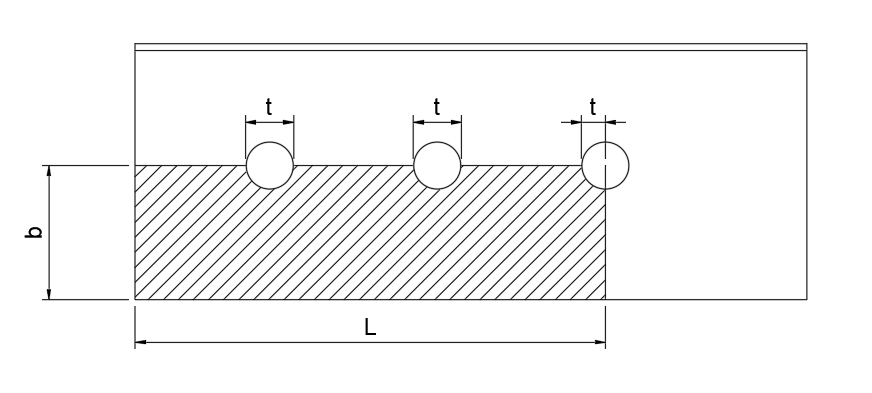
\includegraphics[width=0.5\textwidth]{../images/resumen/bloque}
      \caption{Bloque de corte.}
      \label{fig:bloque}
    \end{figure}

    Por último, utilizando la sección \textbf{J.4.3} del CIRSOC 301 (pág 170), 
    vemos dos casos.

    \textbf{Caso A:} cuando
    $F_u * A_{nt} * (10^{-1}) \geq 0.6 * F_u * A_{nv} * (10^{-1})$, entonces:
    \begin{align*}
      \phi * R_n = \phi * [0.6 * F_y * A_{gv} * F_u * A_{nt}] * (10^{-1})
    .\end{align*}
    \textbf{Caso B:} cuando
    $F_u * A_{nt} * (10^{-1}) \leq 0.6 * F_u * A_{nv} * (10^{-1})$, entonces:
    \begin{align*}
      \phi * R_n = \phi * [0.6 * F_u * A_{nv} * F_u * A_{gt}] * (10^{-1})
    .\end{align*}
\end{description}

\subsection{Chapa de unión}

Es un elemento normalmente utilizado para unir perfiles y columnas. Generalmente
se toma como referencia el bulón más alejado, y tomando dos lineas que salgan
a 30º se obtiene la longitud $L'$, como se muestra en \Cref{fig:chapa}.

\begin{figure}[htpb]
  \centering
  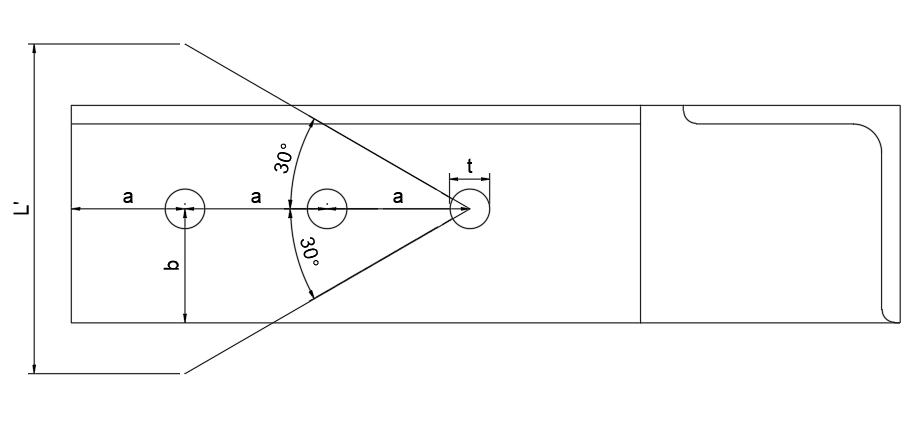
\includegraphics[width=0.8\textwidth]{../images/resumen/chapa}
  \caption{Esquema de chapa.}
  \label{fig:chapa}
\end{figure}

Obteniendo esta longitud, y conociendo el espesor de la chapa $e'$
(normalmente 1/8"), podemos obtener el área bruta y neta como:
\begin{align*}
  A_g &=  e' * L' \\[5pt]
  A_n &= A_g - t * e'
.\end{align*}

Luego, de forma similar a lo hecho para una unión abulonada, debemos verificar
la fluencia en la sección bruta y la rotura en la sección neta, pero no es
necesario verificar bloque de corte.

\section{Compresión áxil}

Cuando evaluamos la compresión axil, es crucial considerar el \textbf{pandeo}. 
Para esto nos valemos de la \textit{teoría de Euler}, que tiene como hipótesis:
\begin{enumerate}
  \item El material es isótropo, homogéneo y elástico.
  \item La barra es perfectamente recta inicialmente y sección constante.
  \item La fuerza de compresión actua a lo largo del eje recto.
  \item Los elementos de la barra son articulaciones perfectas sin fricción, por
    lo que el acortamiento no esta restringido.
  \item Las deformaciones son pequeñas.
  \item Las únicas tensiones son debidas a fuerza áxil.
\end{enumerate}

Vamos a considerar dos tipos de perfiles: barras simples y barras armadas.

\subsection{Pandeo local}

Para poder hacer esto consideramos la sección A-B.5 del Apéndice B del CIRSOC
301. 

Lo primero que debemos encontrar es el factor \textbf{Q}, que es una correción
por \textbf{elementos esbeltos}. La misma es igual a:
\begin{align*}
  Q = Q_s * Q_a
.\end{align*}

Donde $Q_s$ es el menor factor de reducción por pandeo local de los elementos 
comprimidos no rigidizados de la sección transversal, y  $Q_a$ es el factor de
reducción por pandeo local de los elementos comprimidos rigidizados de la
sección transversal.

Consideramos que si la sección solo tiene elementos no rigidizados, $Q_a=1$, y
si solo tiene elementos rigidizados,  $Q_s=1$.

\subsubsection{Elementos no rigidizados $Q_s$}

Para el cálculo de este tipo de elementos utilizamos lo visto en \textbf{A-B.5.3.(a)}
Dependiendo del tipo de perfil, primero debemos verificar si tenemos elementos
esbeltos. Entramos a la \textbf{Tabla B.5.1.} y elegimos el caso que tengamos. 
Luego, buscamos la \textit{relación ancho/espesor} y $\lambda_r$. Entonces, si 
$\lambda_r \leq b/t$, \textbf{tenemos elementos esbeltos}, por lo que es
necesario encontrar el valor de $Q_s$, que en caso contrario, será  $Q_s=1$.

En caso de encontrar que tenemos elementos esbeltos, determinamos un caso del
\textbf{A-B.5.3.(a)} y obtenemos el valor.

\begin{description}
  \item[Viga doble Te] para este caso, en la tabla consideramos el \textbf{Caso 5}, donde vemos que:
    \begin{align*}    
      \text{relación ancho/espesor} =  b / t \\[5pt]
      \lambda_r = 0.64*\sqrt{\frac{E}{F_y / k_c}} 
    .\end{align*}

    Donde el valor de $k_c$ se obtiene como:

    \begin{align*}
      0.35 \leq k_c = \frac{4}{\sqrt{h / t_w}} \leq 0.763
    .\end{align*}

    Verificamos que tenemos elementos esbeltos. Si los tenemos, utilizamos el
    caso C de \textbf{A-B.5.3.(a)}. 
    
    Cuando:
    \begin{align*}
      0.45 * \sqrt{E / F_y} \leq (b/t) \leq 0.91 \sqrt{E / F_y}  \\[5pt]
      Q_s = 1.34 - 0.76*(b / t) * \sqrt{F_y / E} \leq 1 
    .\end{align*}

    Cuando:
    \begin{align*}
      (b / t) \geq 0.91 * \sqrt{E / F_y} \\[5pt] 
      Q_s = \frac{0.53 * E}{\left( F_y * \left(\frac{b}{t}  \right)^2  \right)} \leq 1 
    .\end{align*}
\end{description}

\subsubsection{Elementos rigidizados $Q_a$}

Para el cálculo de éste coeficiente lo debemos hacer de forma \textit{iterativa}
pero primero realizamos la misma verificación que en el paso anterior. Desde la
\textbf{Tabla B.5.1}, en la sección de elementos rigidizados, verificamos si
tenemos elementos esbeltos. De tenerlos, lo primero que hacemos es obtener la 
esbeltez global. Conociendo el valor de k, tenemos:

\begin{align*}
  \lambda &= \frac{k*L}{r} \\[5pt]
  \lambda_c &= \frac{\lambda}{\pi}*\sqrt{\frac{F_y}{E}} 
.\end{align*}

Luego, \textbf{proponemos un valor} de $Q_a$. Un buen valor es 0.8. Luego,
obtenemos, ya habiendo determinado el valor de $Q_s$ anteriormente.
A partir de la sección \textbf{A-B.5.3.b}, dependiendo del tipo de sección,
adoptamos un caso.

Con el valor propuesto, cuando:

\begin{align*}
  \sqrt{Q} &* \lambda_c  \leq 1.5 \\[5pt]
  F_{cr} &= Q*\left( 0.658^{Q*\lambda_c^2} \right)*F_y \tag{A-B.5.15}
.\end{align*}

Cuando:

\begin{align*}
  \sqrt{Q} &* \lambda_c  \geq 1.5 \\[5pt]
  F_{cr} &= \left( 0.\frac{877}{\lambda_c^2} \right) * F_y \tag{A-B.5.16}
.\end{align*}

Luego, adoptamos:

\begin{align*}
  f = \phi_c * F_{cr} = 0.85 * F_{cr}
.\end{align*}

Teniendo este valor, podemos elegir el caso (normalmente Caso B), de 
\textbf{A-B.5.3.(b)}, podemos obtener el valor de $b_e$, que es el ancho
efectivo reducido. Entonces, el área efectiva reducida será:

\begin{align*}
  A_{ef} = A_{g} - \Sigma (b-b_e)*t
.\end{align*}
 
Y se verifica el valor de $Q_a$ como:

 \begin{align*}
   Q_a = \frac{A_{ef}}{A_g}
.\end{align*}

Si la diferencia no es importante, se adopta $Q_a$, en caso contrario, se debe
iterar con un nuevo valor. Si se adopta el valor dado, se prosigue a verificar
el valor de $F_{cr}$ y $R_d$.

\subsection{Columnas simples}

Lo primero que se debe evaluar es el valor de la longitud de pandeo $k*L$. Esto
depende principalmente del coeficiente k. El mismo dependerá de las condiciones
de borde de la columna. Se puede hacer una primera aproximación con lo mostrado
en \Cref{fig:k_aprox}.

\begin{figure}[htpb]
  \centering
  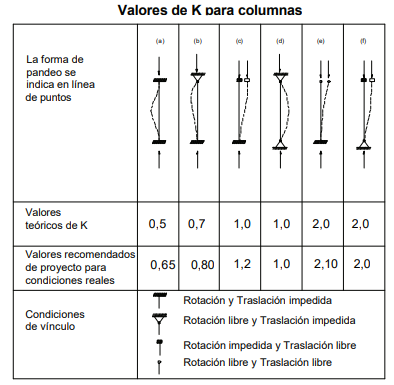
\includegraphics[width=0.8\textwidth]{../images/resumen/k_aprox}
  \caption{Figura 4-15 de CIRSOC 301.}
  \label{fig:k_aprox}
\end{figure}
 
En general, si tenemos \textbf{sistemas indesplazables}, se puede adoptar:

\begin{align*}
  k = 1 \tag{para sistemas indesplazables}
.\end{align*}

Para el caso de \textbf{sistemas desplazables} debemos calcular el mismo a
partir de los nomogramas de \textbf{4.5 (B)} (pág. 133 del PDF).

\subsubsection{Coeficiente k para sistemas desplazables}

Lo primero que se debe hacer es realizar la verificación para reducir por
inelasticidad. Tomando la sección \textbf{C-C.2} de los Comentarios del CIRSOC
301 (pag 81 del PDF), vemos que:

\begin{align*}
  P_{u} / P_{y} \leq 1/3 \hspace{0.25cm} \xrightarrow{\hspace*{0.5cm}} \hspace{0.1cm} \beta = 1 \\[5pt] 
.\end{align*}

En caso contrario, si $P_u / P_y > 1/3$, tenemos:

\begin{align*}
  \beta = -7.38 * (P_u / P_y) * \log \left( \frac{P_u / P_y}{0.85} \right) 
.\end{align*}

Donde $P_u$ es la resistencia requerida de la columna en kN, y $P_y$ la 
resistencia de fluencia de la columna.

\subsubsection{Uso de nomogramas}

Luego de encontrar el valor de $\beta$, debemos encontrar los valores de $G_a$ 
y de $G_b$. En caso de que una de las articulaciones sea empotrada, entonces el
valor de $G_i = 1$. 

Los valores de  $G_i$ se obtienen como:

 \begin{align*}
   G = \frac{\Sigma (\beta * I_c / L_c)}{\Sigma (I_g / L_g)}
.\end{align*}

Donde se consideran todas las barras rigidamente unidas al nudo y contenidas en
el plano de pandeo de la columna considerada, $I_c$ es el momento de inercia de
la columna, $L_c$ la longitud no arriostrada de la columna, $I_g$ el momento
de inercia de la  viga y $L_g$ la longitud no arriostrada de la viga.

Conociendo los dos valores, utilizamos la \textbf{Figura C-C.2.2} (pág 79 de
Comentarios del CIRSOC 301), para obtener el valor de K.

\subsubsection{Cálculo de tensión crítica y verificación}

Luego de conocido el valor de K, debemos encontrar la tensión crítica. Primero,
encontramos la mayor \textbf{esbeltez reducida}. Para esto, comparamos las
\textbf{esbelteces geométricas} de la pieza en sentido X y en sentido Y.

Primero, consideramos la esbeltez geométrica \textit{en dirección x} y
\textit{alrededor del eje y}:
\begin{align*}
  \lambda_y = \frac{k*L}{r_y}
.\end{align*}

Luego, la esbeltez geométrica \textit{en dirección y} y \textit{alrededor del}
\textit{eje y} será:
\begin{align*}
  \lambda_x = \frac{k*L}{r_x}
.\end{align*}

Adoptamos el valor máximo de $\lambda_i$, y obtenemos la esbeltez reducida como:
\begin{align*}
  \lambda_c = \frac{\lambda}{\pi} * \sqrt{\frac{F_y}{E}}  
.\end{align*}

A partir de la sección \textbf{E.2} del CIRSOC 301 (pág 106), tenemos:

\begin{align*}
  F_{cr} &= \left( 0.658^{\lambda_c^2} \right)*F_y \tag{$\lambda_c \leq 1.5$}  \\[5pt]
  F_{cr} &= \left( \frac{0.877}{\lambda_c^2} \right) * F_y \tag{$\lambda_c \geq 1.5$}
.\end{align*}

Conocida la tensión crítica $F_{cr}$, podemos obtener la resistencia nominal y 
la resistencia de diseño de una pieza como:

\begin{align*}
  P_{n} &= A_g * F_{cr} * (10^{-1}) \\[5pt]
  P_{d} &= \phi * P_n
.\end{align*}

En este caso, $\phi=0.85$, ya que es resistencia a la compresión.

\subsection{Columnas armadas}

Las columnas armadas estan conformadas por varios perfiles y generalmente
diagonales. En partícular, consideramos las del Grupo 4, definidas en 
\textbf{A-E.4.2.1.} del CIRSOC 301 (pág 215).

En las mismas consideramos como carga última, tanto el valor de $P_u$ como el de
un momento $M_s$ que comprime a uno de los cordones de perfiles. Entonces, lo
primero es obtener el momento $M_s$.

\subsubsection{Paso 1: obtención de $M_s$}

Para obtener esto es necesario obtener la \textit{esbeltez de la columna armada
como una unidad} $\lambda_o$, a partir de la que podemos obtener su esbeltez 
modificada. Todo esto se hace con respecto al \textbf{eje libre}, que es aquel
que no corta las barras. En el caso analizado será el eje Y.

\begin{figure}[htpb]
  \centering
  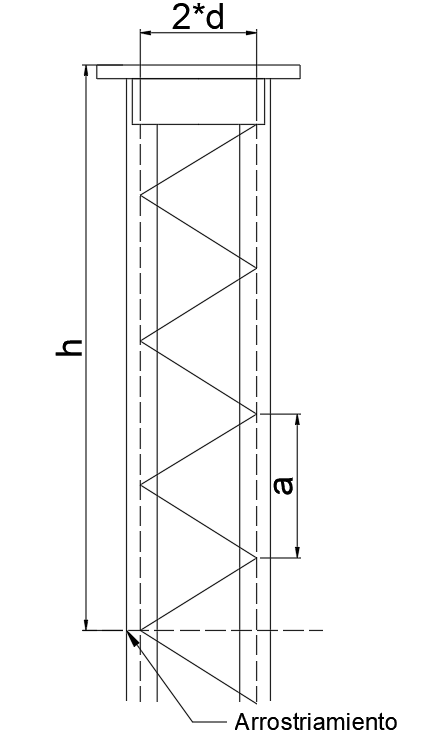
\includegraphics[width=0.4\textwidth]{../images/resumen/armada}
  \caption{Vista de columna armada.}
  \label{fig:armada}
\end{figure}

\begin{figure}[htpb]
  \centering
  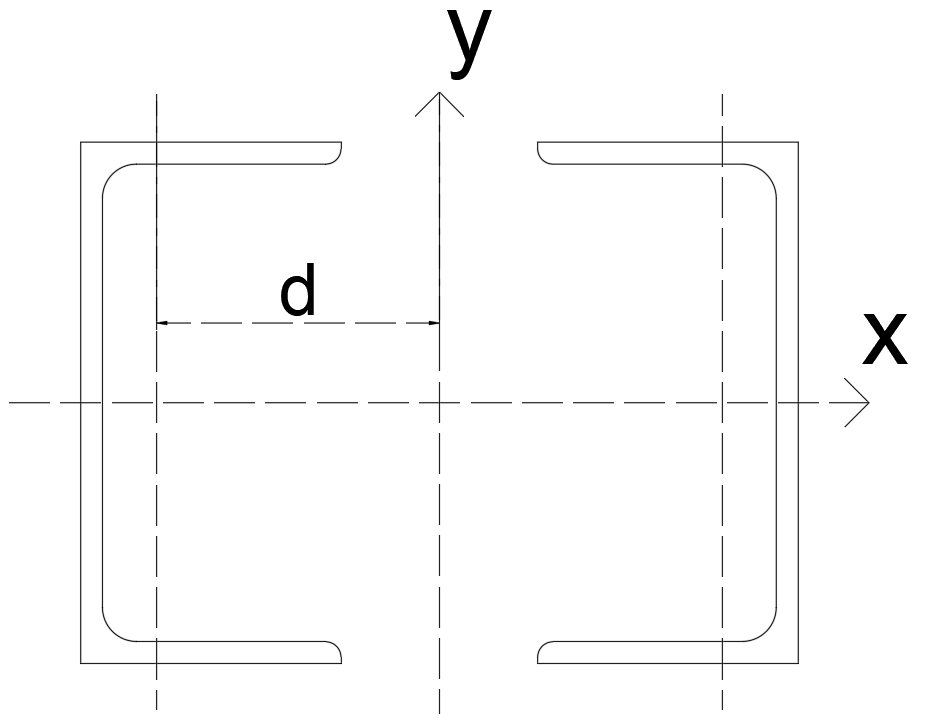
\includegraphics[width=0.5\textwidth]{../images/resumen/armada_trans}
  \caption{Sección de columna armada}
  \label{fig:armada_trans}
\end{figure}

Considerando una columna de un cordón de perfiles, con dos perfiles como se 
muestra en \Cref{fig:armada_trans}, podemos obtener el radio de giro del cordón
mediante el teorema de Stainer, y considerando la inercia \textit{paralela} al
eje libre, que en este caso sería Y.

Primero obtenemos la inercia, y luego el radio de giro como:

\begin{align*}
  I_{py} &= I_g + A_g * d^2 \\[5pt]
  r_c &=  \sqrt{\frac{I_{py}}{A_g}} 
.\end{align*}

Por último, obtenemos el valor de $\lambda_0$ como:

\begin{align*}
  \lambda_0 = \frac{k*L}{r_c}
.\end{align*}

Luego, necesitamos obtener el valor de $\lambda_1$, que es un valor auxiliar que
se relaciona con la rigidez a corte de las vigas de celosía. Esta se determina
según cuestiones de configuración de la celosía y geometría, y puede ser
determinada mediante la \textbf{Figura A-E.4.2} del CIRSOC 301 (pág 217).

Determinados estos dos valores, obtenemos la esbeltez modificada $\lambda_m$
como:

\begin{align*}
  \lambda_m = \sqrt{\lambda_0^2 + \lambda_1^2} 
.\end{align*}

Con este valor podemos obtener $P_{cm}$:

\begin{align*}
  P_{cm} = \frac{\pi^2 * E * A_g}{\lambda_m^2} *(10^{-1})
.\end{align*}

También debemos considerar una excentricidad debido a una deformación inicial,
que se obtiene como:

\begin{align*}
  e_o = \frac{k*L}{500} \text{, en cm}
.\end{align*}

Entonces podemos obtener el momento $M_s$ como:

 \begin{align*}
   M_s = \frac{P_u*e_o}{1-P_u /P_{cm}} * (10^{-2})\text{, en kNm}
.\end{align*}

\subsubsection{Paso 2: determinación de carga última $P_{u1}$}

En este paso debemos considerar tanto las cargas últimas $P_u$,  $M_u$ y  también
el momento $M_s$. Esto lo hacemos como:

 \begin{align*}
   P_{u1} = \frac{P_u}{n} + \frac{M_s}{n_1*h} * (10^2)
.\end{align*}

Siendo $n$ el número de barras de la columna armada (n=2 ó n=4), y $n_1$ el
número de barras del cordón considerado ($n_1$ = 1 ó $n_1$ = 2).

\subsubsection{Paso 3: determinación de resistencia de diseño $P_d$}

Esta determinación se hace con la siguiente ecuación:

\begin{align*}
  P_d = \phi * F_{cr} * A_{g1} * (10^{-1}) 
.\end{align*}

Donde el $F_{cr}$ se determinara según ciertas condiciones. Primero debemos
determinar que esbeltez geometrica debemos adoptar. En principio, consideramos
dos:

\begin{enumerate}
  \item \textit{Esbeltez local:} es la esbeltez que se da entre en dirección del
    eje debil de cada perfil, pero que se encuentra arriostrado debido a las 
    vigas de celosía. 
  \item \textit{Esbeltez global:} es la esbeltez de la pieza en la dirección
    paralela al eje libre, y que normalmente se encuentra arriostrada.
\end{enumerate}

Si consideramos la \Cref{fig:armada}, y considerando las esbleteces nombradas,
tenemos:

\begin{align*}
  \lambda_{x} &= \frac{k*h}{r_x} \tag{General} \\[5pt]
  \lambda_{c_1} &= \frac{L_1}{r_y} \tag{Local}
.\end{align*}

Esto es generalmente así, ya que se arriostra con celosía generalmente la
dirección más débil, y se lo arriostra entre columnas en la otra dirección para
reducir el valor de $h$, que es la distancia libre.

Adoptando el menor de ambos valores, tenemos:

\begin{align*}
  \lambda = \frac{\lambda_x}{\pi} * \sqrt{\frac{f_y}{E}}   
.\end{align*}

Luego, con este valor cálculamos el valor de $F_{cr}$:

\begin{align*}
  F_{cr} &= \left( 0.658^{\lambda_c^2} \right)*F_y \tag{$\lambda_c \leq 1.5$}  \\[5pt]
  F_{cr} &= \left( \frac{0.877}{\lambda_c^2} \right) * F_y \tag{$\lambda_c \geq 1.5$}
.\end{align*}

Conocida la tensión crítica $F_{cr}$, podemos obtener la resistencia nominal y 
la resistencia de diseño de una pieza como:

\begin{align*}
  P_{n} &= A_g * F_{cr} * (10^{-1}) \\[5pt]
  P_{d} &= \phi * P_n
.\end{align*}

\subsubsection{Paso 4: verificación de diagonales}

Para este paso se considera la sección \textbf{A-E.4.2.1 (b)} del CIRSOC 301 
(pág. 218). Lo primero es la determinación de $\beta$, que se hace como:

\begin{align*}
  \beta = \frac{\pi}{400} * \left( \frac{1}{1-P_u / P_{cm}} \right) 
.\end{align*}

Entonces, encontramos el corte último $V_{eu}$, que se obtiene como:

\begin{align*}
  V_{eu} = \beta * P_u + V_u
.\end{align*}

Este esfuerzo debe ser proyectado a las diagonales, que se puede hacer mediante
la siguiente formula:

\begin{align*}
  D_u = \frac{V_{eu}}{2} * \frac{d}{h}
.\end{align*}

Donde los valores de $d$ y $h$ son los determinados en la 
\textbf{Figura A-E.4.2.} del CIRSOC 301 (pág. 217).

Luego, verificamos la resistencia a compresión de la misma. Tomando el Caso 3 de
la \textbf{Figura C.2.4} del CIRSOC 301 (pág. 92), y obteniendo el área del 
perfil de la diagonal y su radio de giro mínimo, obtenemos:

\begin{align*}
\lambda_{c\text{(diag)}} = \frac{k*L_d}{r_{min}} * \frac{1}{\pi} * \sqrt{\frac{F_y}{E}} 
.\end{align*}

Luego, obtenemos la tensión crítica $F_{cr}$ como ya se describió, y se determina
el valor de $P_d$ y se verifica lo siguiente:

\begin{align*}
  P_d = 0.85 * F_{cr} * A_{g \text{(diag)}} \geq D_u
.\end{align*}

\subsubsection{Paso 5: verifiación de la presilla}

Esta parte se hace según la sección \textbf{A-E.4.3.1} del CIRSOC 301 (pág 221),
que dice que en los extremos de las barras armadas se deberán colocar
\textit{presillas}, que restringen que los extremos de las mismas se desvien. Las
mismas deberán satisfacer la siguiente condición:

\begin{align*}
  \frac{n_p * l_p}{h} \geq \frac{10 * I_1}{a}
.\end{align*}

con $h$ y $a$ según la  \textbf{Figura A-E.4.3} (pág ), y donde $I_1$ es la 
inercia del cordón con respecto al eje paralelo al eje libre analizado,  $n_p$,
el número  de planos de presillas y $I_p$ el momento de inercia de una presilla.

De la ecuación podemos despejar lo siguiente:

\begin{align*}
  I_p \geq \frac{10 * h * I_1}{a * n_p}
.\end{align*}

De lo anterior, sabemos los valores de $I_1$ (normalmente $I_y$), $h$ y de $a$.
En principio, además podemos adoptar el número de presillas como 2 (una en la
parte inferior, y otra en la parte superior), por lo que podemos determinar el
valor de $I_p$.

Luego, debemos adoptar un espesor comercial de planchuela de acero, que puede
ser considerado como 1/8" o 0.635cm, que denominamos $t$. Entonces, despejamos:

 \begin{align*}
  I_p  &= \frac{b*h^3}{12} \\[5pt]
  h &= \sqrt[3]{\frac{12*I_p}{t}} 
.\end{align*}

Con este valor podemos adoptar una altura de precilla, con lo que queda
terminado la verificación de una columna armada.
\end{document}
